%!TEX root = report.tex
\chapter{Evaluation}

\section{Accuracy}
How accurate are the predictions?
\subsection{Compare predictions to real data}
We can compare the predictions generated to the live bus arrivals data stored in the arrivals table. We can calculate the standard deviation of the difference in the predicted time and actual arrival time. This value will be the direct indicator of the accuracy of the predictions.

\section{Correctness and Performance}
\subsection{Tool}
\par We used \textit{siege}\cite{siege} to conduct the load test of our API endpoints. Our aim was to test the number requests the server could handle reliably at one time, and the response time it took.

\par \textit{Siege} takes in the number of users, the delay time between each page load, the test running time, and the list of URLs to send requests to as parameters. It then simulates the user behaviours to fire requests to the list of given URLs. At the end of the test, \textit{Siege} generates a report for the test, including metrics such as the transaction rate, and the response time of the target URLs.

\subsection{Preparation}
\par We generated a list of API URLs with random parameters for testing. We then ran the siege tests by fixing the test running time to be 1 minute, with 1 second of delay between each page load.

\subsection{Test for Correctness}
\par We first tested for the correctness of our API endpoints. This involves firing requests with random day of the week and hour of day, route, run, and starting bus stop code to check whether the server can return a response correctly.

\par At this stage, we found some specific URLs that resulted in a 500 error code, and debugged the backend code to return correct results. For example, this happened when we requested for a reference travel time for a bus route at an hour out of its operating time. As there was no corresponding entry in the databases, we fixed the code by returning an empty list by default.

\par After we received 200 status code for all requests in a few test runs consistently, we proceeded to perform the load tests by fixing the day of the week and hour of the day to be the current values when the test was run.

\subsection{Load Test for Performance}
\par We found out that currently, the server could reliably handle about 150 users to send requests concurrently, with an average response time of 15.78 seconds. Figure \ref{fig:performance} shows the results of our tests.

\begin{figure}
\centering
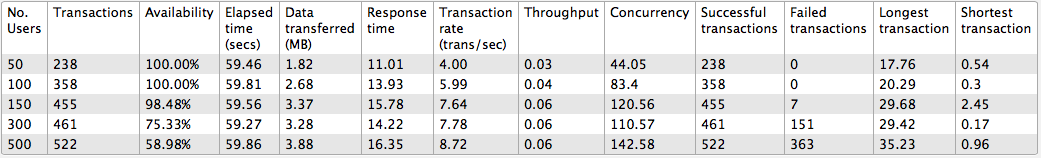
\includegraphics[width=\textwidth]{figures/performance.png}
\caption{\label{fig:performance} Result of Performance Test with Siege}
\end{figure}

\todo[inline]{plot graph from results}

\section{User feedback on UI}
\par On the
How effective is it at warning delay?

